%%%%%%%%%%%%%%%%%%%%%%%%%%%%%%%%%%%%%%%%%%%
%%% DOCUMENT PREAMBLE %%%
\documentclass[12pt]{article}
\usepackage[T1]{fontenc}
%\usepackage{natbib}
\usepackage{url}
\usepackage[utf8x]{inputenc}
\usepackage{amsmath}
\usepackage{graphicx}
\graphicspath{{images/}}
\usepackage{parskip}
\usepackage{fancyhdr}
\usepackage{vmargin}
\usepackage{mathtools}
\usepackage{enumitem}
\setmarginsrb{2 cm}{2.5 cm}{2 cm}{2.5 cm}{1 cm}{1.5 cm}{1 cm}{1.5 cm}
\usepackage{subfigure}
\usepackage{blindtext}
\usepackage{tcolorbox}
\tcbuselibrary{minted,breakable,xparse,skins}

\definecolor{bg}{gray}{0.95}
\DeclareTCBListing{mintedbox}{O{}m!O{}}{%
  breakable=true,
  listing engine=minted,
  listing only,
  minted language=#2,
  minted style=default,
  minted options={%
    linenos,
    gobble=0,
    breaklines=true,
    breakafter=,,
    fontsize=\small,
    numbersep=8pt,
    #1},
  boxsep=0pt,
  left skip=0pt,
  right skip=0pt,
  left=25pt,
  right=0pt,
  top=3pt,
  bottom=3pt,
  arc=5pt,
  leftrule=0pt,
  rightrule=0pt,
  bottomrule=2pt,
  toprule=2pt,
  colback=bg,
  colframe=orange!70,
  enhanced,
  overlay={%
    \begin{tcbclipinterior}
    \fill[orange!20!white] (frame.south west) rectangle ([xshift=20pt]frame.north west);
    \end{tcbclipinterior}},
  #3}

\title{Rapport de projet}
% Title
\author{
Yannis Elrharbi-Fleury \\
Yuan Fangzheng
}						
% Author
\date{25/05/2021}
% Date

\setcounter{secnumdepth}{4}

\makeatletter
\let\thetitle\@title
\let\theauthor\@author
\let\thedate\@date
\makeatother

\pagestyle{fancy}
\rhead{\thedate}
\lhead{\thetitle}
\cfoot{\thepage}
%%%%%%%%%%%%%%%%%%%%%%%%%%%%%%%%%%%%%%%%%%%%
\begin{document}
\bibliographystyle{IEEEtran}
%%%%%%%%%%%%%%%%%%%%%%%%%%%%%%%%%%%%%%%%%%%%%%%%%%%%%%%%%%%%%%%%%%%%%%%%%%%%%%%%%%%%%%%%%

\begin{titlepage}
	\centering
    \vspace*{0.5 cm}
   
\includegraphics[scale = 0.075]{Images/logo_SU.jpeg}\\[1.0 cm]	% University Logo
\begin{center}    \textsc{\Large   Sorbonne Université}\\[2.0 cm]	\end{center}% University Name
	\textsc{\Large Résolution de problème : problème d'ordonnancement}\\[0.5 cm]				% Course Code
	\rule{\linewidth}{0.2 mm} \\[0.4 cm]
	{ \huge \bfseries \thetitle}\\
	\rule{\linewidth}{0.2 mm} \\[1.5 cm]
	
	\begin{minipage}{0.4\textwidth}
		\begin{flushleft} \large
		\emph{Encadrant :}\\
		Evripidis Bampis\\
		\textbf{\Large }
			\end{flushleft}
			\end{minipage}~
			\begin{minipage}{0.4\textwidth}
            
			\begin{flushright} \large
			\emph{Étudiants :}\\
			\theauthor
		\end{flushright}
           
	\end{minipage}\\[2 cm]
	
\end{titlepage}

%%%%%%%%%%%%%%%%%%%%%%%%%%%%%%%%%%%%%%%%%%%%%%%%%%%%%%%%%%%%%%%%%%%%%%%%%%%%%%%%%%%%%%%%%
\newpage																		
<<<<<<< HEAD

\setlength{\parindent}{2ex}

\section*{Introduction}

L’apprentissage par renforcement [1] consiste en une recherche heuristique, dans un environnement donné, d’une stratégie permettant de maximiser une récompense. \par

Dans certains environnement, cette approche est moins performante que des algorithmes évolutionnaires. De plus, il est démontré que certaines méthodes d’entraînement tirent leur efficacité de transformations de l’espace d’apprentissage. \\

Cette recherche étant propre à l’environnement, et par construction s’effectuant dans un espace en grande dimension, il est nécessaire de s’intéresser au développement d’outils permettant de mieux comprendre ce processus et d’expliquer ces phénomènes. \\

Lors de notre projet, nous avons travaillé à l’amélioration de deux outils de visualisation mis au point les années précédentes [8]. Ils permettent d’obtenir des aperçus du paysage de valeur autour d’un agent. \\

Lors de nos travaux, nous avons complètement réécrit le code de ces outils pour le rendre plus modulable et plus clair pour l’utilisateur. De plus, nous avons ajouté de nouvelles fonctionnalités de visualisation. \\

Dans ce rapport nous rappelons le fonctionnement des outils développés, puis détaillons notre implémentation de ceux-ci en présentant les nouvelles fonctionnalités. Nous démontrons ensuite l'intérêt de ces derniers grâce à des exemples d'utilisation, pour enfin évoquer des idées d'améliorations futures à apporter aux outils. \\

\newpage

=======
>>>>>>> 15bdf415c9ad437b54126b223afd17aaa8f76c6c
\renewcommand*\contentsname{Table des Matières}
\tableofcontents 

\newpage
<<<<<<< HEAD
\section{Principe de fonctionnement des outils de visualisation}

Le principe de fonctionnement des outils développés les années précédentes repose sur une méthode d’échantillonnage de l’espace d’apprentissage selon des droites. \\

Les outils développés permettent d'obtenir un aperçu en deux dimensions de l'espace d'apprentissage d'un modèle, alors en grande dimension (de la taille du réseau de neurones). \\

Le premier outil, \emph{étude de gradient} \ref{gradient}, permet d'observer la trajectoire du modèle lors de son apprentissage. Le second, \emph{Vignette} \ref{vign}, permet d'observer le paysage de valeur autour du modèle. \\

La sortie de ces outils est constituée d’un ensemble de lignes de pixels. Chaque ligne est une direction tirée dans l’espace d’apprentissage, le pixel en son centre correspond au modèle à partir duquel elle est tirée. \\

La direction est ensuite échantillonnée à une fréquence entrée par l’utilisateur. La valeur d'un échantillon, quantifiée par une carte de couleur, correspond à la récompense obtenue en cette position. \\

% IMAGE d'une seule ligne
\begin{figure}[htp]
    \centering
    
\includegraphics[width=10cm]{Images/Ligne}
    \caption{Un exemple de ligne composant la sortie des outils, une droite discrétisée puis coloriée en fonction de la récompense obtenue}
    \label{fig:ligne1}
\end{figure}

Nous présentons maintenant leur principe de fonctionnement, et le format de leur sortie. \\

\subsection{Etude de gradient} \label{gradient}.

Le premier outil, \emph{étude de gradient}, permet de suivre la descente de gradient d’un modèle. \\

% IMAGE GradientStudy from above
\begin{figure}[!htp]
    \centering
    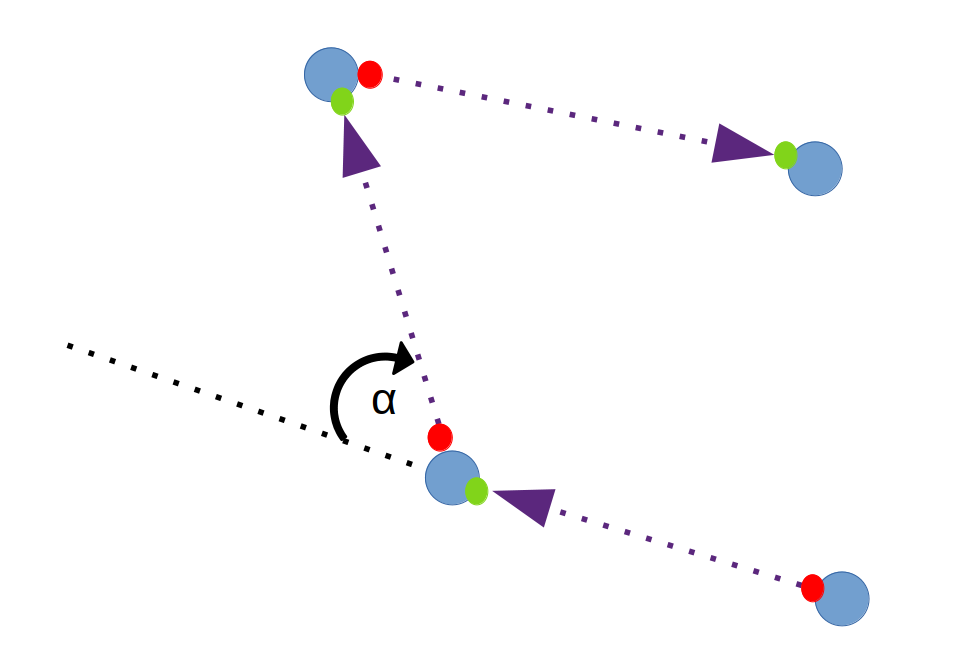
\includegraphics[width=8cm]{Images/gradientStudy_dessus}
    \caption{Descente de gradient en 2D, le modèle se déplace dans l'espace d'apprentissage en marquant un angle $\alpha$ entre deux pas.}
    \label{fig:gradientStudyAbove}
\end{figure}

Il consiste à prendre comme lignes les directions prises par la descente de gradient à chaque pas. Pour avoir une idée du déplacement effectué entre deux pas, on indique la position relative des modèles sur les droites : une pastille rouge pour la position au pas précédent, une verte pour la position au pas actuel. \\

De plus, le produit scalaire entre deux directions est représenté sur le côté droit de la sortie. L'utilisateur y lit une image du changement d'angle du modèle lors de la descente de gradient. \\

% IMAGE GradientStudy
\begin{figure}[!htp]
    \centering
    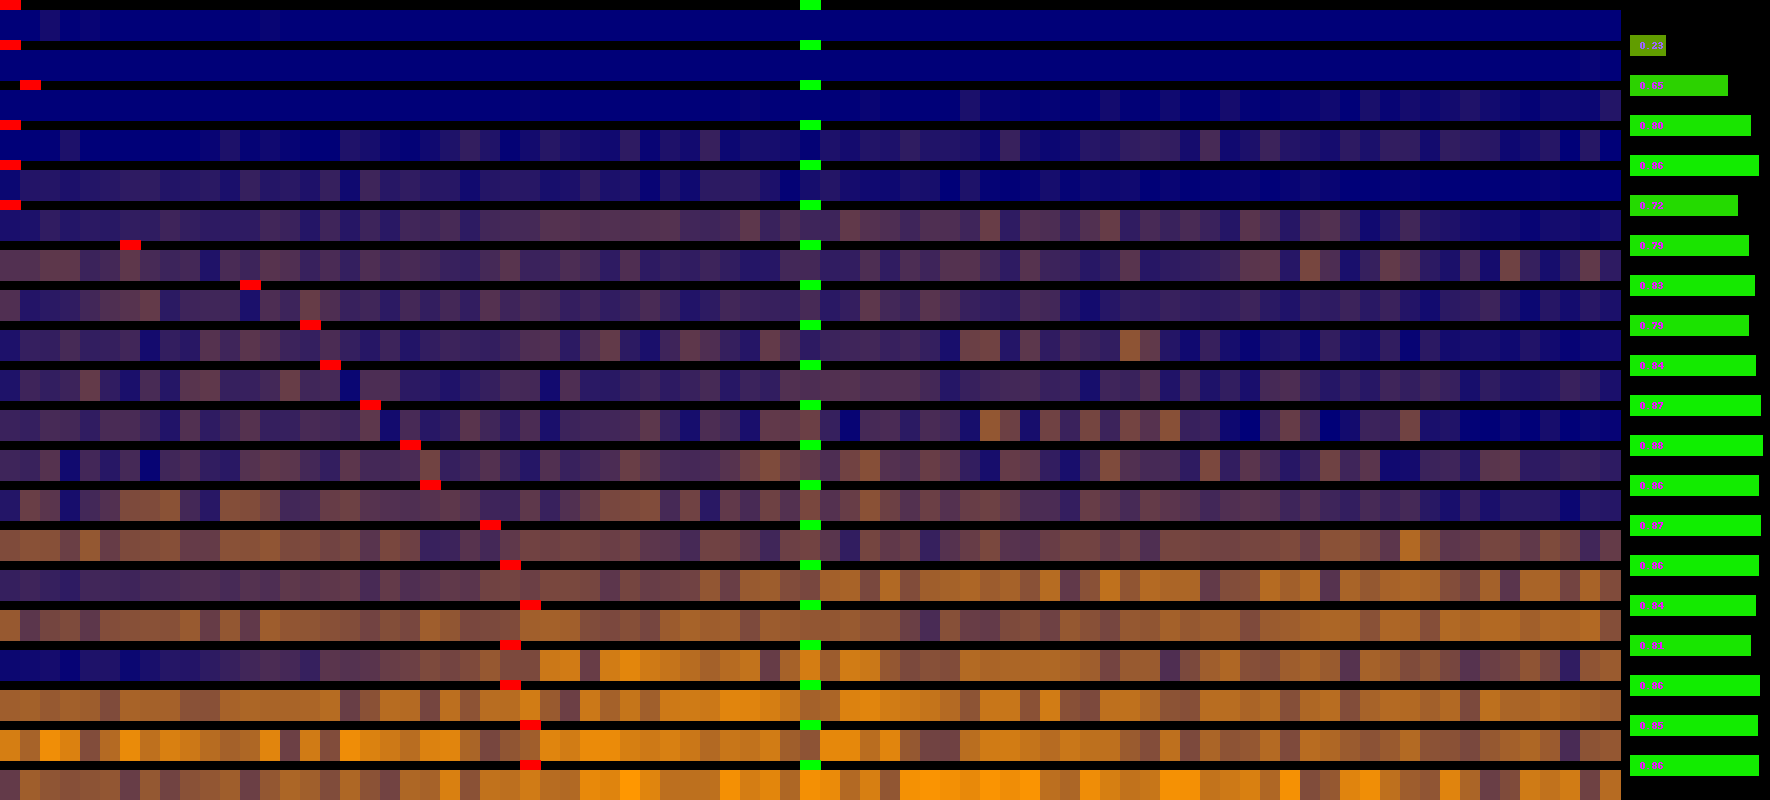
\includegraphics[width=10cm]{Images/gradientStudy}
    \caption{Un exemple de sortie de l'étude de gradient, algorithme SAC [2], environnement \emph{Pendulum} [12] entraînement enregistré tous les 500 pas de 500 à 10.000. La sortie se lit de haut en bas, plus la récompense est grande plus la couleur est claire. De haut en bas, on observe que le modèle se déplace de moins en moins rapidement vers une zone à forte récompense. De plus, l'angle entre chaque direction est faible car le produit scalaire, indiqué sur la droite, est proche de 1. Il pourrait être intéressant d'effectuer une étude de gradient autour des premiers pas, car on observe que le changement de direction est plus le important entre le pas 500 et le pas 1.000.}
    \label{fig:gradientStudy}
\end{figure}

Ainsi, cet outil donne un aperçu en deux dimensions de la trajectoire prise par un modèle lors de son apprentissage (en n dimensions, n étant la taille du réseau de neurones). \\

\newpage
\subsection{Vignette} \label{vign}
=======
%%%%%%%%%%%%%%%%%%%%%%%%%%%%%%%%%%%%%%%%%%%%%%%%%%%%%%%%%%%%%%%%%%%%%%%%%%%%%%%%%%%%%%%%%
\setlength{\parindent}{2ex}
>>>>>>> 15bdf415c9ad437b54126b223afd17aaa8f76c6c

\section{Introduction}
Ce projet porte sur l'étude de solutions au problème d'ordonnancement. \par

Étant donné $N$ tâches et $1$ machine, il s'agit de trouver un ordonnancement de ces tâches minimisant la somme de leur temps de complétude (minimiser le temps d'attente total). \par

La machine ne connaît pas forcément leur durée d'exécution réelle. \par

Dans ce rapport, nous étudions et mesurons la qualité de plusieurs solutions en fonction de l'erreur de prédiction. \\

<<<<<<< HEAD
% IMAGE Vignette real
\begin{figure}[htp]
    \centering
    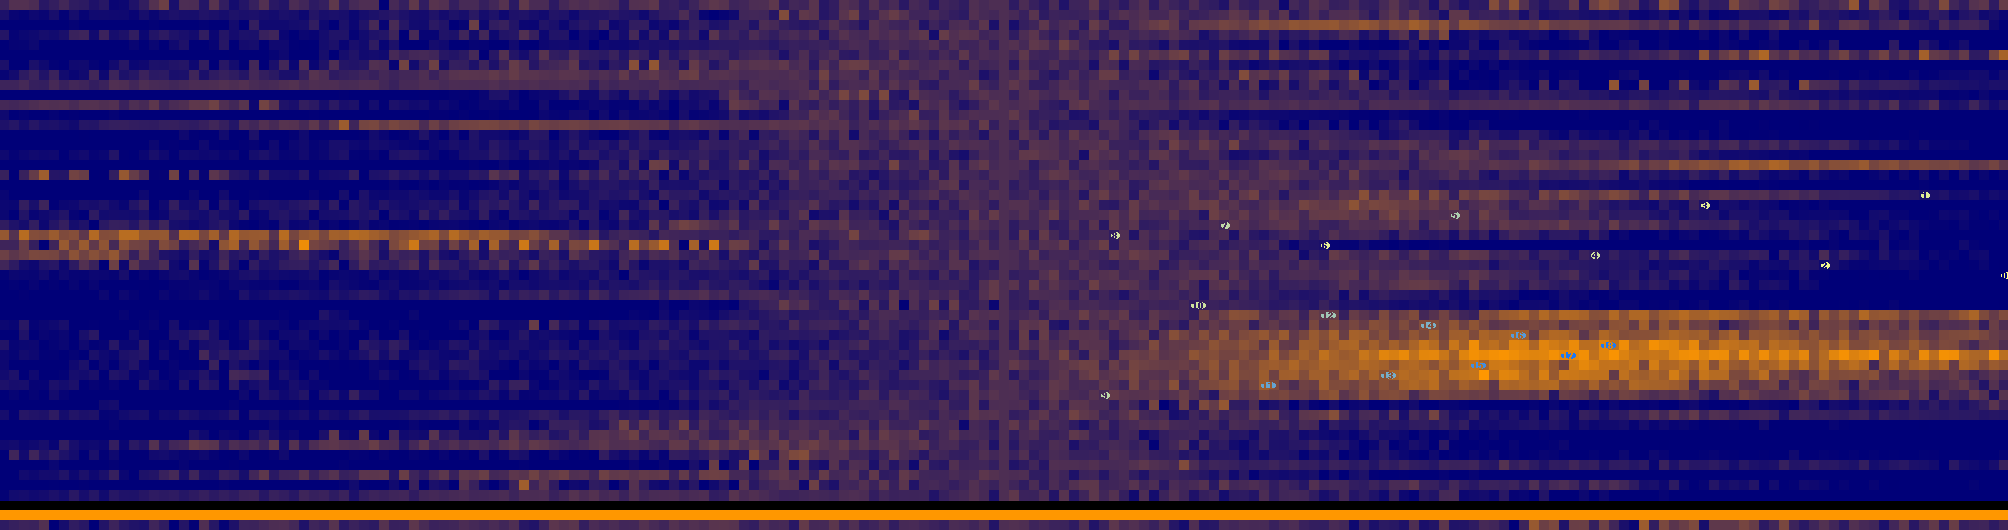
\includegraphics[width=15cm]{Images/Vignette_pendulum}
    \caption{Un exemple de sortie de \emph{Vignette}, algorithme SAC  [2], environnement \emph{Pendulum} entraîné pendant 5.000 pas, 50 directions tirées aléatoirement. La politique entrée est située au centre de la \emph{Vignette}. Autour du modèle, on observe un environnement bruité, de moyenne récompense. De plus, certaines zones en bordure de la boule observée sont clairement à faible récompense, tandis que deux zones à proximité offrent une meilleur récompense. On en déduit que ce sont deux zones dans lesquelles la descente de gradient est susceptible de converger.}
    \label{fig:vignettePendulum}
\end{figure}
=======
Le code est écrit en Python et sera fourni en annexe.
>>>>>>> 15bdf415c9ad437b54126b223afd17aaa8f76c6c

\newpage
\section{Structure du programme}

Nous avons naturellement opté pour une approche orientée objet du problème.

\subsection{Les distibutions}
La classe \emph{Distribution} représente un ensemble de distributions de probabilité et leurs paramètres. \\

Lors de son instanciation, elle prend en argument des fonctions permettant de générer un tuple de valeurs. \\

La méthode \emph{sample} renvoie un tuple contenant :
\begin{itemize}
	\item une durée réelle
	\item une durée erreur de prédiction
	\item un instant d'arrivée
\end{itemize}

<<<<<<< HEAD
Dans cette partie, nous détaillons chacune de ces phases.

\subsection*{Portage à \emph{stable-baselines-3}}

Lors de nos travaux, nous avons été contraints de réécrire le code des outils. En effet, celui-ci était écrit pour fonctionner sur un environnement particulier (\emph{Mujoco Swimmer}) sous l’algorithme TD3 [7]. \\

Nous avons procédé à un portage vers la librairie \emph{Stable-baselines-3} [11].
, comportant un ensemble fiable d’implémentations d’algorithmes d’apprentissage par renforcement en PyTorch [13]. Le code de cette librairie est accessible sur github et celle-ci propose une documentation détaillée de ses implémentations. \\

Ainsi, pour chacun des outils, il est possible pour l’utilisateur de changer facilement l’algorithme d’apprentissage, ses hyper-paramètres et l’environnement utilisé. \\

\subsection{Phase de préparation}

Avant toutes choses, pour fonctionner, les outils ont besoin de recevoir en entrée un modèle entraîné sous forme de réseau de neurones. \\

Grâce à leur implémentation sous \emph{stable-baselines-3 (SB3)} [11]., les outils peuvent recevoir n'importe quel réseau de neurones au format PyTorch [13]. \\

Nous proposons un exemple d'application de \emph{SB3} [11].
 dans le fichier \emph{trainModel.py}. L'utilisateur peut alors entraîner un réseau de neurones sous l'environnement souhaité, en sauvegardant les étapes de l'apprentissage à un rythme choisi. \\

De plus, l'étude portant sur une descente de gradient, l'utilisateur peut fournir en entrée de \emph{Vignette} une liste de politiques. Il peut alors observer la position relative de chacune des politiques de la liste avec la politique centrale de la \emph{Vignette}. \\

% IMAGE politiques comparaison
\begin{figure}[htp]
    \centering
    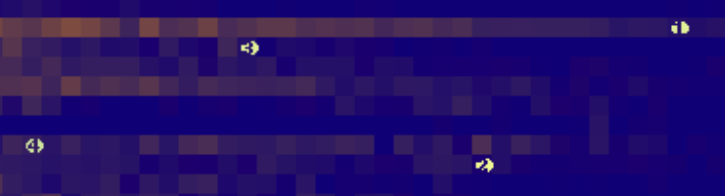
\includegraphics[width=10cm]{Images/politiques_entrees_vignette}
    \caption{Extrait d'une \emph{Vignette} affichant des politiques d'entrée}
    \label{fig:exempleEntree}
\end{figure}

Nous détaillons comment ces politiques d'entrée sont prises en compte lors du calcul de \emph{Vignette} dans la partie suivante. \\

\subsection{Phase de calcul}

\emph{L'étude de gradient} prend en entrée un ensemble de politiques, correspondant à la progression de la descente de gradient pour le modèle entraîné. Comme décrit précédemment, il calcule un suivi de la descente de gradient effectuée par le modèle. \\

% IMAGE gradientStudy Swimmer
\begin{figure}[htp]
    \centering
    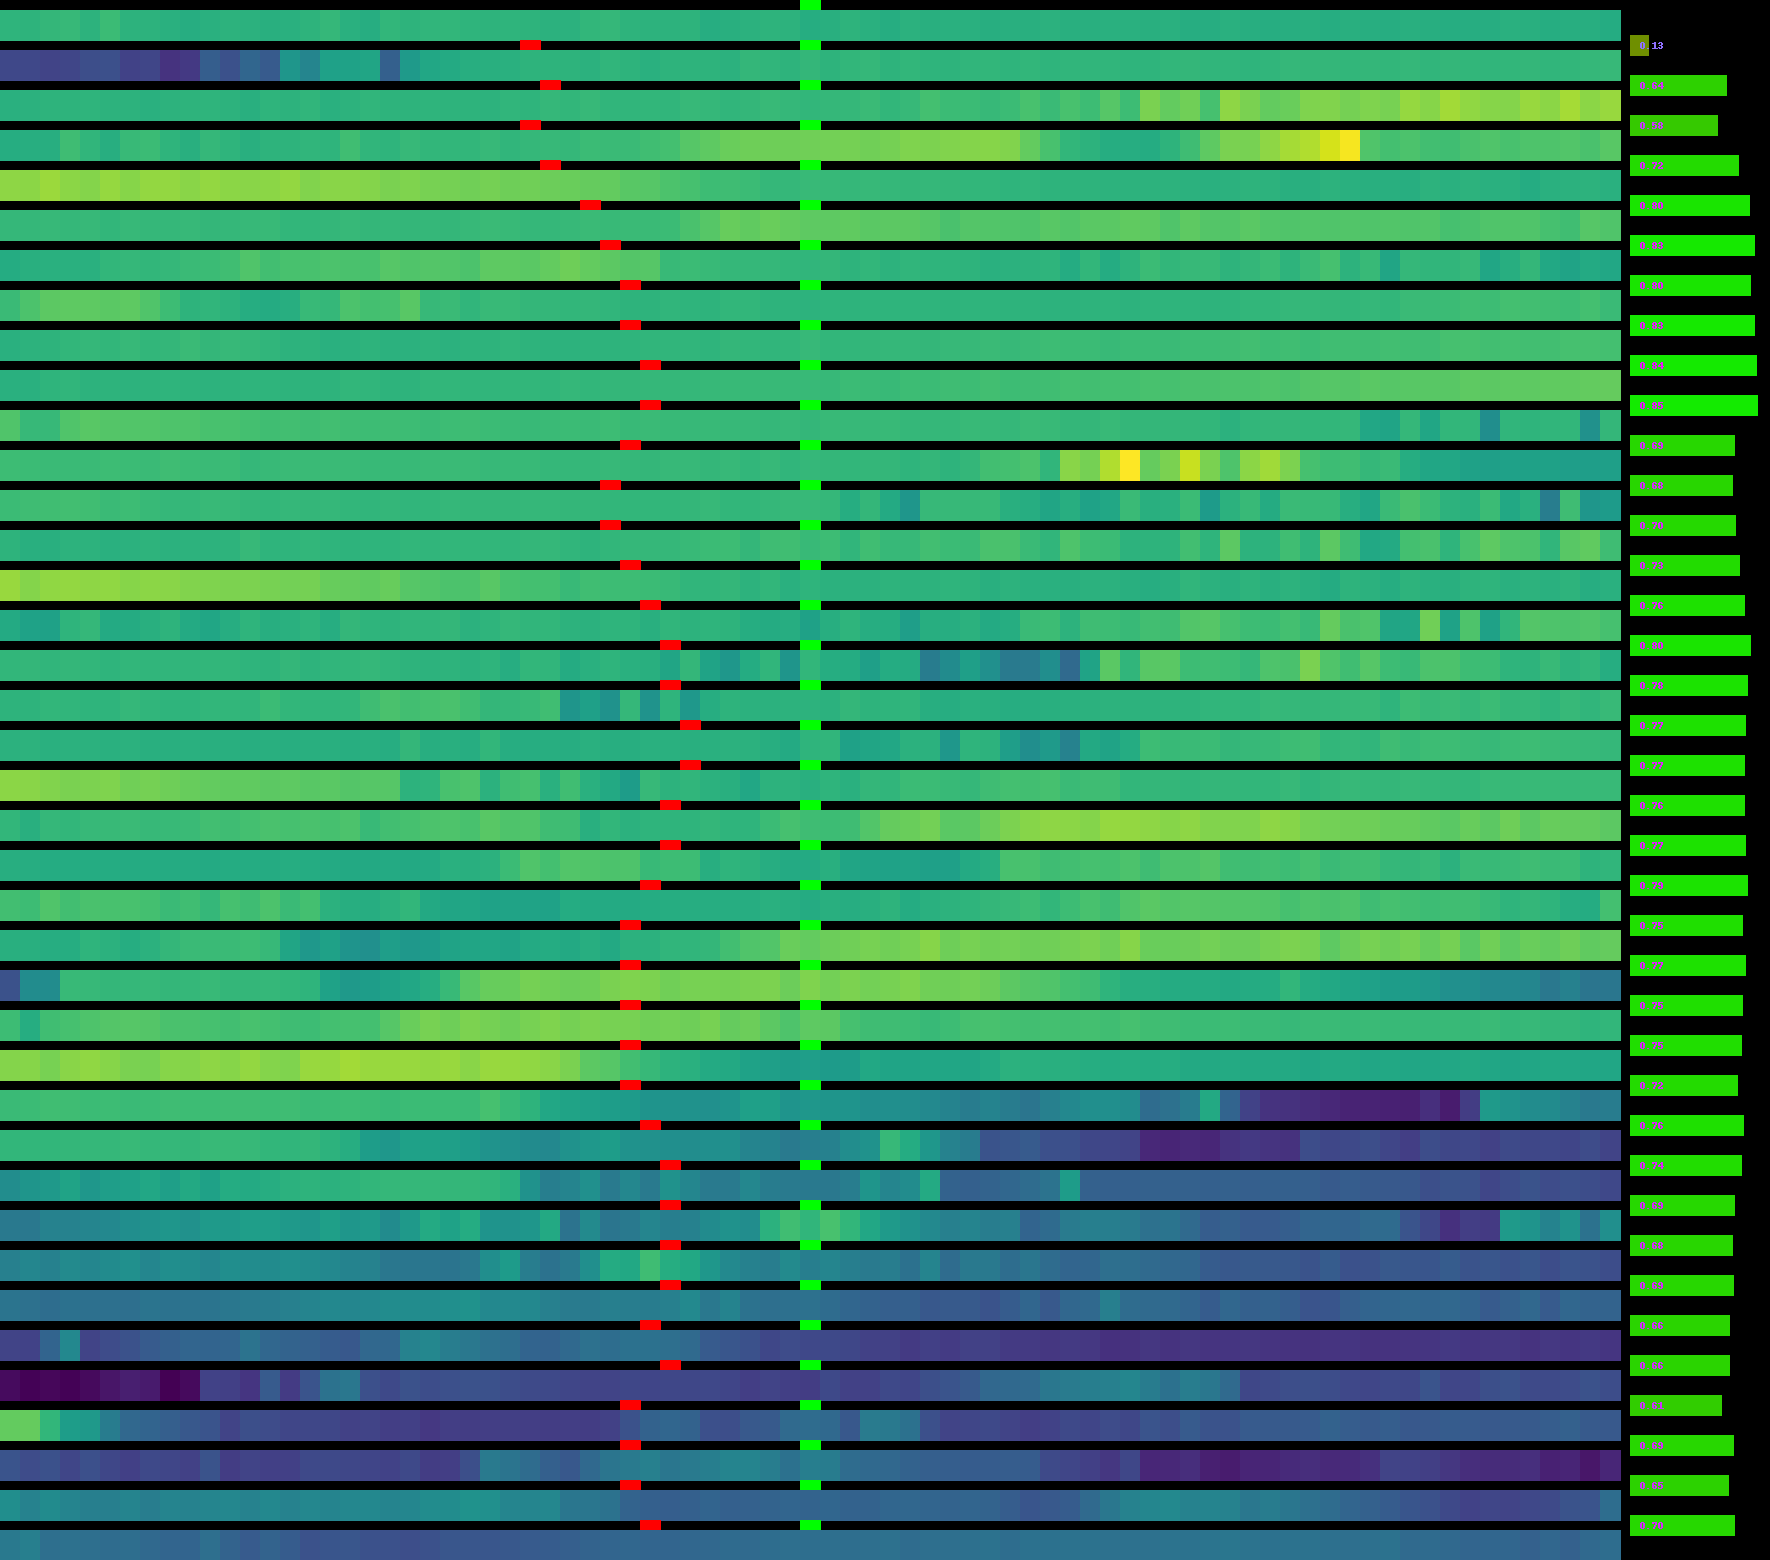
\includegraphics[width=15cm]{Images/gradientStudy_swimmer}
    \caption{Etude de gradient sur Swimmer 250 pas à 10.000 pas sauvegardé tous les 250 pas, algorithme SAC [2]. On note tout d'abord que la normalisation des couleurs s'effectue sur les valeurs extrêmes observées, ce point sera abordé dans la section \hyperref[sec:affichage]{Phase d'affichage}. On remarque que le modèle se déplace en tâtonnant dans une zone uniforme en suivant globalement la même direction (faible angle entre chaque ligne), il finit même par réduire sa récompense. On en déduit que l'initialisation de Swimmer s'effectue dans une zone à gradient uniforme, ce qui fait partir la descente de gradient dans une mauvaise direction.}
    \label{fig:gradientStudy}
\end{figure}

Pour \emph{Vignette}, la possibilité d'entrer une liste de politiques à situer dans la sortie rajoute des étapes de calculs. Leur prise en compte s'effectue en deux étapes. \\

La première étape consiste à ajuster la fréquence d'échantillonnage des droites. \\

En effet, on rappelle que l'utilisateur donne en argument de \emph{Vignette} une fréquence d'échantillonnage. Cette fréquence correspond à la résolution de chaque ligne. Par conséquent, \emph{Vignette} dispose d'une portée limitée. On ne peut observer qu'un aperçu de la boule ayant pour centre le modèle central, et un rayon résultant de la résolution choisie. \\

Il est possible que des politiques d'entrée soient en dehors de cette boule. Nous avons donc fait le choix d'imposer une baisse automatique de la fréquence d'échantillonnage de façon à atteindre toutes les politiques. \\

\newpage
 
% IMAGE vignette portée
\begin{figure}[htp]
    \centering
    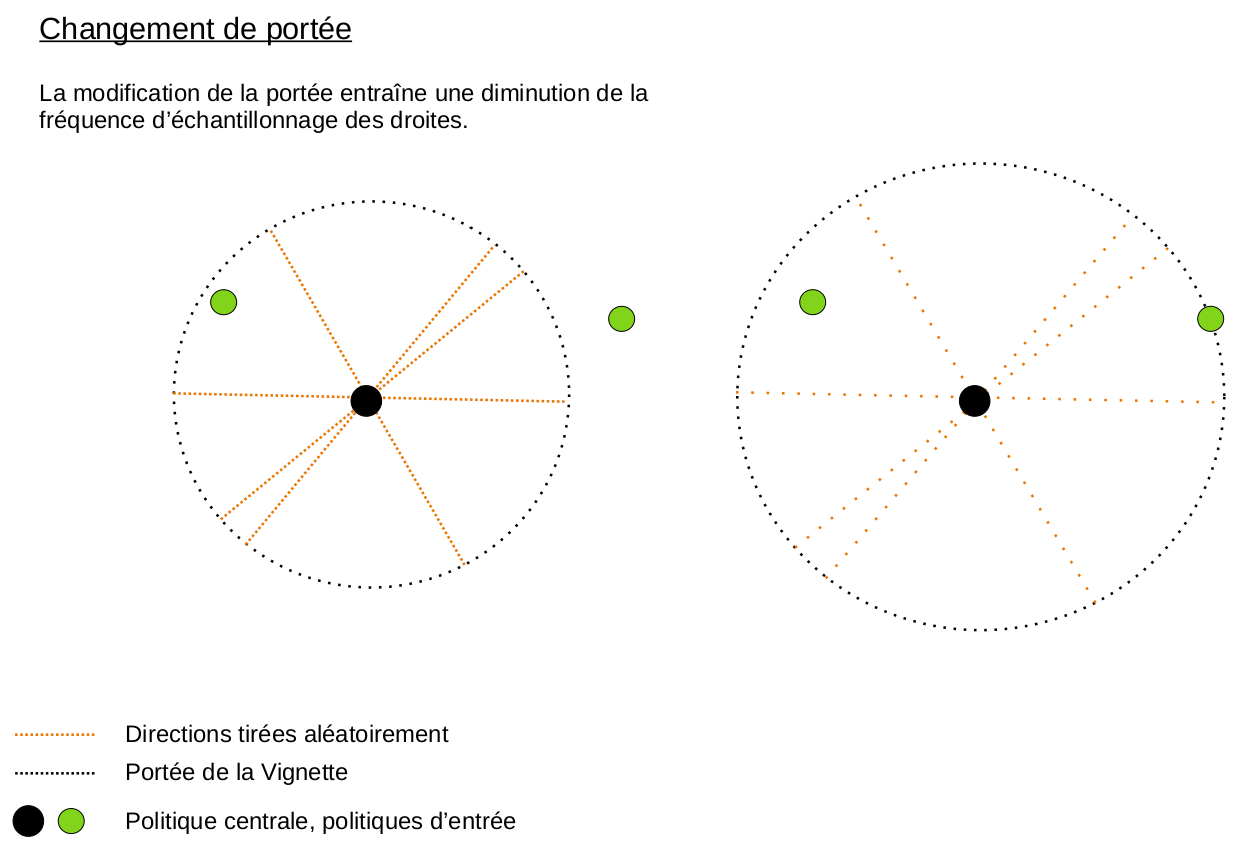
\includegraphics[width=18cm]{Images/vignette_portee1}
    \caption{Première étape : ajustement de la portée}
    \label{fig:vignettePortee}
\end{figure}

La seconde étape consiste à insérer les directions passant par les politiques d'entrée dans le résultat final. \\

Le nombre de lignes tirées (la hauteur de la Vignette) étant un paramètre de l'utilisateur, il convient de remplacer certaines de ces lignes (donc directions) par celles correspondant aux politiques d'entrée. \\

Pour que l'introduction de ces politiques bouleverse le moins possible la Vignette d'origine, on insère les directions correspondantes à la place des directions qui en étaient les plus proches. \\

% IMAGE vignette directions
\begin{figure}[htp]
    \centering
    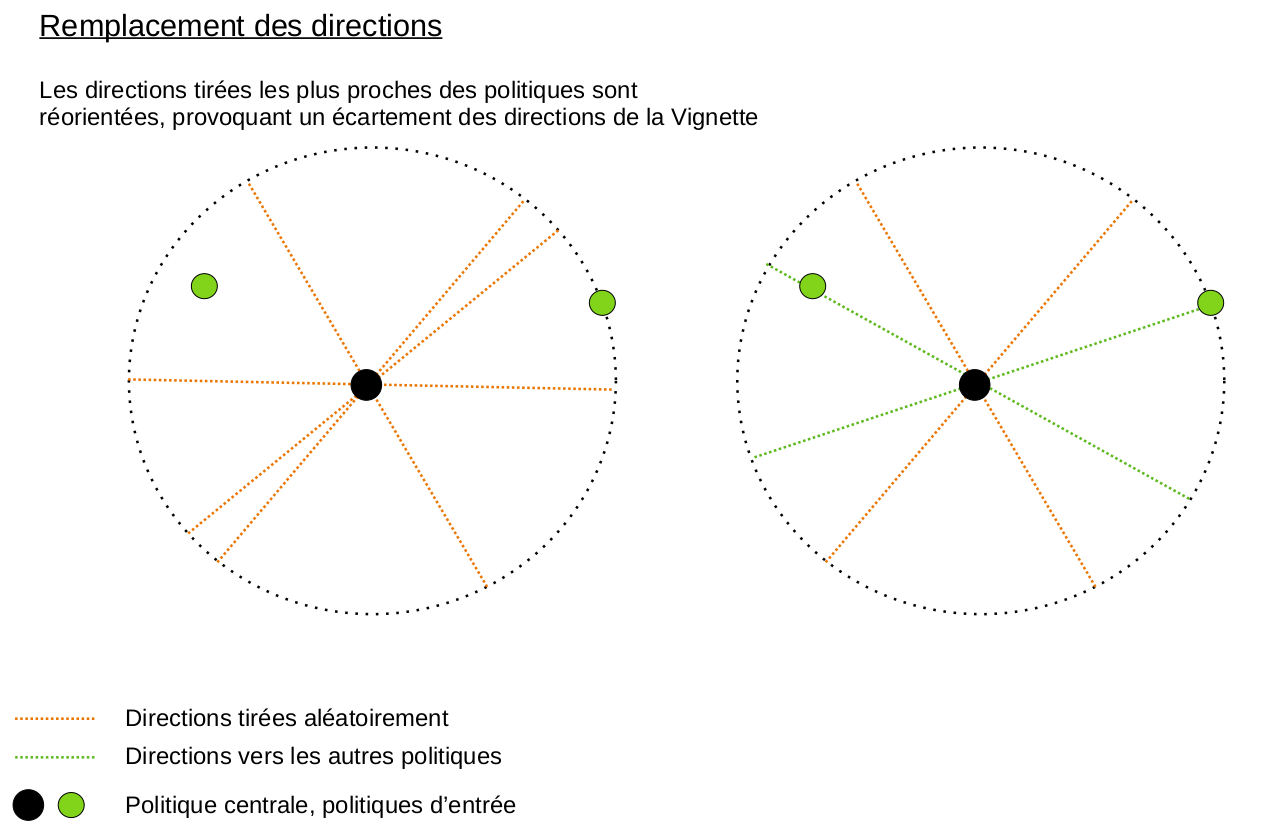
\includegraphics[width=18cm]{Images/vignette_portee2}
    \caption{Seconde étape : insertion des directions}
    \label{fig:vignettePortee}
\end{figure}

\newpage 
On constate dans l'exemple de la \hyperref[fig:vignettePortee]{figure 10} que cette étape a tendance à écarter les directions les unes des autres. \\

Cela a pour inconvénient de provoquer des discontinuités dans la détection de structures. Au contraire, l'utilisateur pourrait préférer concentrer les directions dans des faisceaux, permettant un meilleur niveau de détail autour de directions particulières. C'est un point abordé dans la partie \hyperref[sec:future]{Travaux futurs} du rapport. \\

Au lieu de choisir la direction la plus proche, une solution pourrait être de prendre la direction la plus isolée et la remplacer par la direction vers la politique. \\

C'est un problème flagrant dans notre représentation 2D simplifiée de l'espace d'apprentissage. Mais en réalité, le nombre de directions tirées est bien inférieur à la dimension de l'espace, ce qui réduit l'importance du problème. \\

\subsection{Phase de sauvegarde}

Une fois les calculs effectués, les données sont sauvegardées dans un objet de type \emph{SavedVignette} ou \emph{SavedGradient}. Chacun de ces objets garde en mémoire les directions ayant servi aux calculs, la valeur des récompenses pour chaque pixel. \\

Cette approche permet un traitement ultérieur des données si l'utilisateur le souhaite, cependant celles-ci prennent beaucoup de place en mémoire. \\

Nous utilisons une compression au format \emph{.xz} (algorithmes \emph{LZMA/LZMA2} [16]. Bien qu'il soit relativement lent pour la compression, il est très rapide en décompression. \\

Cela le rend idéal pour notre application : la lenteur de compression est négligeable par rapport au temps de calcul des outils (quelques secondes contre quelques heures), mais la rapidité de décompression est parfaite car l'utilisateur sera amené à fréquemment charger les résultats (pour faire des essais de modification des attributs par exemple). \\

La taille d'un fichier sauvegardé est de l'ordre de 100Mb. \\

\subsection{Phase d'affichage}
\label{sec:affichage}

Tout comme dans la version des années précédentes, nous offrons la possibilité d'afficher les résultats en tant qu'image 2D. Grâce à la fonctionnalité de sauvegarde, nous avons pu implémenter une gestion des palettes de couleur. \\

Nous avons constaté que cette gestion des couleurs était utile. En effet, elle permet aux personnes malvoyantes de régler le contraste des couleurs. De plus, certains écrans ont du mal à distinguer les faibles variations d'intensité de couleur entre les pixels. \\
=======
%% DECRIRE CHOIX DE DISTRIBUTION

\subsection{Les tâches}
La classe \emph{Task} représente une tâche, dont les attributs sont générés à partir d'un objet de type \emph{Distribution}. \\

Elle possède notamment comme attributs :
\begin{itemize}
	\item un ensemble de durée : durée réelle, durée prédite (générées à partir de \emph{Distribution})
	\item un état : \emph{paused, running, finished, not available}
	\item un curseur \emph{currentStep} permettant d'avancer dans l'exécution de la tâche
	\item un numéro d'identification 
\end{itemize}
>>>>>>> 15bdf415c9ad437b54126b223afd17aaa8f76c6c

Une tâche possède trois méthodes :
\begin{itemize}
	\item \emph{hasFinished} : renvoie si la tâche est achevée ou non
	\item \emph{forward} : exécute la tâche d'un pas de temps, renvoie une exécution de \emph{hasFinished}
	\item \emph{restart} : réinitialise la tâche à son état initial
\end{itemize}

\subsection{Les machines}
Notre idée était de créer une classe \emph{Machine} représentant une machine capable de travailler sur un ensemble de tâches. Les différents algorithmes que nous présenterons dans la partie suivante en héritent. \\

Chaque machine possède notamment comme attributs :
\begin{itemize}
	\item des dictionnaires de tâches à différents états : \emph{allTasks, workingTasks, pausedTasks, finishedTasks}
	\item une vitesse d'exécution
	\item une horloge donnant le temps de la machine
	\item une clée d'affichage (une fonction lmabda) permettant de trier les tâches de la machine lors de son affichage
\end{itemize}

<<<<<<< HEAD
% IMAGE Vignette 3D
\begin{figure}[htp]
    \centering
    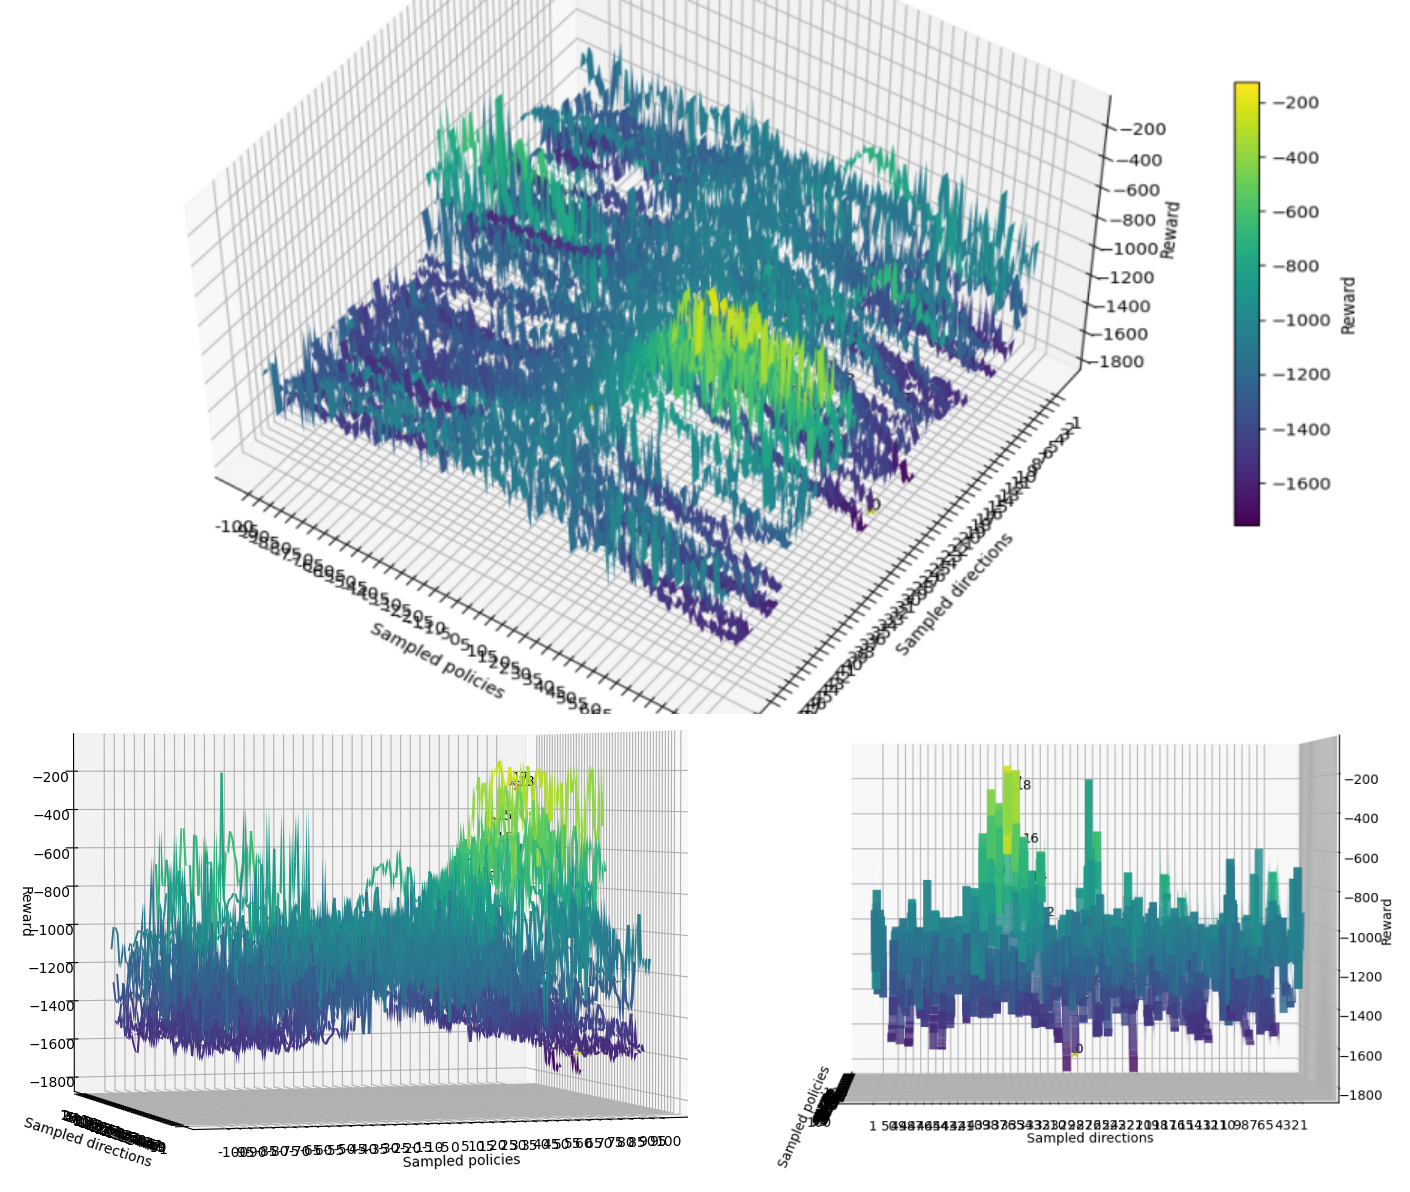
\includegraphics[width=15cm]{Images/vignette_3D}
    \caption{Vignette 3D, algorithme SAC [2], environnement \emph{Pendulum} (p:\pageref{second}) entraîné pendant 5.000 pas, 50 directions tirées aléatoirement. Il est plus facile d'appréhender les structures présentes dans le paysage de valeur. Le caractère bruité du paysage est flagrant.}
    \label{fig:vignette3D}
\end{figure}
=======
Ainsi, \emph{Machine} possède plusieurs méthodes concernant ses tâches : ajouter ou supprimer des tâches; démarrer, mettre en pause ou terminer une tâche. \\
>>>>>>> 15bdf415c9ad437b54126b223afd17aaa8f76c6c

Elle possède aussi des méthodes permettant de les traîter :
\begin{itemize}
	\item une méthode de travail \emph{work} faisant travailler les tâches sur un pas de temps de la machine
	\item une méthode abstraite de traitement \emph{run} traîtant les tâches avant chaque étape de travail, elle permet d'introduire l'algorithme de la machine
	\item une méthode de démarrage \emph{boot} démarrant la machine et la faisant tourner jusqu'à ce que toutes ses tâches soient terminées
\end{itemize}

\subsection{Les machines parallèles}
La classe \emph{Parallel} fonctionne de façon analogue à \emph{Machine}, à ceci près qu'elle ne fournit pas le travail aux tâches elle même. \\

Le travail sur les tâches est effectué par deux machines (\emph{Prediction} et \emph{Round-Robin}) que possède \emph{Parallel}, les exécutant avec une vitesse $\lambda$ et $1 - \lambda$.

\newpage
\section{Implémentation des algorithmes}

Grâce à notre refléxion claire sur les structures de données, nous avons pu facilement implémenter les aglorithmes demandés. \\

Dans cette partie, nous nous contenterons de présenter le fonctionnement de ceux-ci. Nous étudierons leurs performances dans la prochaine section. \\

Les algorithmes suivant héritent de \emph{Machine} ou \emph{Parallel} et ne font que surchager la méthode \emph{run}. \\

\subsection{Algorithme optimal : Shortest processing time}

L'agorithme \emph{SPT} est un algorithme optimal pour ce problème. \\

Il connaît la durée réelles des tâches et les exécute de la plus courte à la plus grande. \\ 

\begin{mintedbox}{python}
    def run(self, step):
        if len(self.workingTasks) == 0:
            nextTask = sorted(list(self.pausedTasks.values()), key=lambda x:x.realLength)[0]
            self.startTask(nextTask)
        return self.work(step)
\end{mintedbox}

Sa méthode \emph{run} est claire : si aucune tâche n'est en cours d'exécution, alors la machine exécute la plus courte.

\subsection{Exécution par prédiction}

Pour l'algorithme \emph{Prediction}, la machine n'a pas accès aux durées réelles des tâches. Elle ne connait que leur durée prédite, avec par conséquent une certaine erreur. \\

<<<<<<< HEAD
Le groupe d'Hector Kohler et Damien Legros [15]. cherche à comprendre les différences de résultats donnés par deux méthodes de recherche de politique sur l'environnement \emph{Pendulum}. \\

La première méthode étudiée est la \emph{Cross entropy method} [5], la seconde est une méthode de descente de gradient \emph{Policy gradient}. \\

Après avoir remarqué que la distance entre politiques successives est grande dans le cas de \emph{CEM} [5] et petite dans l'autre cas, ils ont decidé d'utiliser \emph{Vignette} pour directement observer l'espace des politiques. Ils l'ont intégré à leur code, et cela leur a permis de constater que l'initialisation des réseaux de neurones était située dans une zone plate en terme de récompense. \\
=======
\begin{mintedbox}{python}
    def run(self, step):
        if len(self.workingTasks) == 0:
            nextTask = sorted(list(self.pausedTasks.values()), key=lambda x:x.predLength)[0]
            self.startTask(nextTask)
        return self.work(step)
\end{mintedbox}

La méthode est quasiment identique à l'algorithme précédent, à ceci près que les tâches sont triées en fonction de leur durée prédite.

\subsection{Round-Robin}
>>>>>>> 15bdf415c9ad437b54126b223afd17aaa8f76c6c

L'algorithme \emph{Round-Robin} partage son travail de façon égale entre les tâches. \\

Cet algorithme est utile dans le cas où les prédictions sont mauvaises, car il possède un rapport de compétitivité $\max_i {\frac {A(I)} {OPT(I)}}$ de $2$. \\

Notre implémentation se déroule en deux phases : l'initialisation (toutes les tâches démarrent) et l'exécution (\emph{run}). \\

\begin{mintedbox}{python}
    def _initRun(self):
        for task in self.allTasks.values():
            self.startTask(task)
            
    def run(self, step):
        if self.currentTime == 0:
            self._initRun()

        self.speed = self.initSpeed / len(self.workingTasks)
        return self.work(step)
\end{mintedbox}

Il suffit de changer la vitesse de la machine en fonction du nombre de tâches restantes à chaque pas de temps.

\subsection{Exécution parallèle}

Comme vu précédemment, \emph{Parallel} exécute \emph{Predicition} et \emph{Round-Robin} aux vitesses $\lambda$ et $1 - \lambda$. \\

Ainsi, lors de l'initialisation de la machine, on définit ses sous-machines :
\begin{mintedbox}{python}
        self.speed = speed
        self.prediction = Prediction(speed * lmb, key)
        self.roundRobin = RoundRobin(speed * (1-lmb), key)
\end{mintedbox}

Les deux machines possèdent les même tâches en référence, et travaillent ensemble à leur avancement. \\

La méthode \emph{run} prend la forme suivante :
\begin{mintedbox}{python}
    def run(self, step):
        self.currentStep += step

        self.finishTasks()

        if not bool(self):
            self.prediction.run(step)
            self.roundRobin.run(step)

        return bool(self)
        
    def __bool__(self):
        return bool(self.prediction) or bool(self.roundRobin)
\end{mintedbox}

Avec les méthodes \emph{bool} renvoyant si les machines ont fini leur exécution ou non.

\subsection{Exécution parallèle dynamique}
%% A FINIR DE REDIGER

Nous avons eu l'idée d'expérimenter une version de machine parallèle au $\lambda$ dynamique. \\

Lorsqu'une tâche s'achève, on regarde à intervalle régulier la différence entre le temps d'exécution prédit, et le temps réellement effectué. \\

On utilise la formule suivante : $\lambda' = e^{-\epsilon_m}$ avec $\epsilon_m$ la moyenne de l'erreur observée. \\

\begin{mintedbox}{python}
    def updateLmb(self):
        if len(self.finishedTasks) != 0 and len(self.finishedTasks) % 5 == 0:
            meanDiff = np.mean([abs(task.currentStep - task.predLength) for task in self.finishedTasks.values()])
            newLmb = np.exp(-meanDiff*self.coef)
    
            self.prediction.speed = self.speed * newLmb
            self.roundRobin.initSpeed = self.speed * (1-newLmb)
            self.historyLmb.append(newLmb)

    def finishTasks(self):
        super().finishTasks()
        self.updateLmb()
\end{mintedbox}

On s'attend alors à observer un déplacement exponentiel du premier ordre des performances de la machine vers celles de \emp{Round-Robin}. \\

Il s'agit de rajouter un coefficient $\alpha$ dans l'exponentielle pour adapter la vitesse de convergence de $\lambda$. \\

\newpage
<<<<<<< HEAD
\section*{Conclusion}

Lors de ce projet, nous avons enrichi les outils développés les autres années. Après les avoir portés à la librairie \emph{stable-baselines-3}, nous les avons rendus plus faciles d'utilisation en reprenant le code à partir de zéro. \\

Il est désormais plus facile pour un utilisateur de comprendre leur principe de fonctionnement et leur architecture, notamment à l'aide du cahier des charges (\emph{user-manual}), de ce rapport et des nombreux commentaires détaillant l'exécution du code. \\

Grâce à leur implémentation sous \emph{SB3} et à l'approche objet lors de leur développement, ceux-ci sont aisément modulables et utilisables dans le cadre d'autres projets. \\

Ainsi, de futurs utilisateurs peuvent ajouter de nouvelles fonctionnalités sans avoir à modifier la structure des données. \\

Enfin, ils pourront s'inspirer de notre code pour développer de nouveaux outils de visualisation 2D ou 3D d'un espace de grande dimension, tels que la méthode des faisceaux introduite précédemment \\


\section{Réferences} \label{second}
[1] R. S. Sutton et A. G. Barto, Reinforcement learning: an introduction. Cambridge (Mass.),
Etats-Unis d’Amérique: The MIT Press, 2018. \label{[1]} \newline
[2] T. Haarnoja et al., « Soft Actor-Critic Algorithms and Applications », ArXiv181205905 Cs
Stat, janv. 2019, Consulté le: févr. 26, 2021. [En ligne]. Disponible sur:
http://arxiv.org/abs/1812.05905   \label{[2]} \newline
[3] R. S. Sutton et A. G. Barto, Reinforcement learning: an introduction. Cambridge (Mass.),
Etats-Unis d’Amérique: The MIT Press, 2018.\label{[3]} \newline
[4] O. Chapelle et M. Wu, « Gradient descent optimization of smoothed information retrieval
metrics », Inf. Retr., vol. 13, n
o 3, p. 216-235, juin 2010, doi: 10.1007/s10791-009-9110-3.\label{[4]} \newline
[5] Z. Botev, D. Kroese, R. Rubinstein, et P. L’Ecuyer, « Chapter 3. The Cross-Entropy
Method for Optimization », in Handbook of Statistics, vol. 31, 2013,p.35 59. \label{[5]} \newline
[6] P-T. De Boer, D.P Kroese, S. Mannor, and R.Y. Rubinstein. A tutorial on the cross-entropy method. Annals of Operations Research, 134(1):19–67, 2005.\label{[6]} \newline
[7] TD3 : https://www.researchgate.net/publication/341648433\_Twin-Delayed\_DDPG\_A\_Deep\_Reinforcement\_Learning\_Technique\_to\_Model\_a\_Continuous\_Movement\_of\_an\_Intelligent\_Robot\_Agent \label{[7]} \newline
[8] Rapport des années précédentes : https://github.com/DevMaelFranceschetti/PAnd\_Swimmer/blob/master/paper\_study\_Swimmer.pdf. \label{[8]} \newline
[9] Projet des années précédentes : https://github.com/DevMaelFranceschetti/PAnd\_Swimmer \label{[9]}\newline
[10] Pendulum : https://pendulum.eustace.io/docs/ \label{[10]}\newline
[11] Stable-baselines 3 : https://stable-baselines.readthedocs.io/en/master/  \label{[11]}\newline
[12] Mujoco : http://www.mujoco.org/ \label{[12]}\newline
[13] Librairie PyTorch : https://pytorch.org/  \label {[13]}\newline
[14] Algorithme LZMA : https://fr.wikipedia.org/wiki/LZMA \label{[14]}\newline
[15] Projet Androide de Hector Kohler et Damien Legros : https://github.com/KohlerHECTOR/PANDROIDE \label{[15]}\newline 
[16] Algorithme LZMA : https://en.wikipedia.org/wiki/Lempel\%E2\%80\%93Ziv\%E2\%80\%93Markov\_chain\_algorithm \label{[16]} \newline

\newpage
\section{Annexe : mode d'emploi}
=======

\section{Test du bon fonctionnement des modèles}
    \subsection{Modèle Prédiction}
    \begin{itemize}
        \item[1]\includegraphics[width=15cm]{trace_0_pred.png} \\
        À l'instant 0 toutes les tâches ne sont pas disponibles.
        
        \item[2]\includegraphics[width=15cm]{trace_1_pred.png}
        
        À l'instant 6, la tâche 1 et 2 devienne disponibles, Prédiction réussi à sélectionner la tâche qui a la moins durée prédite.
        
        \item[3] \includegraphics[width=15cm]{trace_2_pred.png} 
        
        À l'instant 17, la tâche 1 est terminée. Ensuite la tâche 0 a été sélectionnée.
        
        \item[4]  \includegraphics[width=15cm]{trace_3_pred.png}
        
        Toutes les tâches sont terminées à l'instant 42.
    
    \end{itemize}
    
    \subsection{RR}
    \begin{itemize}
        \item[1]\includegraphics[width=15cm]{trace_0_rr.png}
        
        À l'instant 6, la tâche 7 a été sélectionné et allouée une vitesse de 1.
        
        \item[2]\includegraphics[width=15cm]{trace_1_rr.png}
        
        À l'instant 9, toutes les tâches sont exécutées avec une vitesse 0.2.
        
        \item[3]\includegraphics[width=15cm]{trace_2_rr.png}
        
        À l'instant 37, la tâche 7 est terminée. Les tâches restantes ont une vitesse 0.25.
        
        \item[3]\includegraphics[width=15cm]{trace_3_rr.png}
        
        À l'instant 76 toutes les tâches sont terminées.
        
    \end{itemize}

    \subsection{SPT}
    
    \begin{itemize}
        \item[1]\includegraphics[width=15cm]{trace_0_spt.png}
        
        À l'instant 6, la tâche 1 a été sélectionnée.
        
    \end{itemize}
    
    \subsection{Parallèle}
    
    \begin{itemize}
        \item[1]\includegraphics[width=15cm]{trace_0_para.png}
        
        À l'instant 1, la tâche 1 a été sélectionnée par Prédiction.
        
        Donc à l'instant 2, la tâche 1 a été exécutée 0.5*0.5 + 0.5 = 0.75, alors que la tâche 2 a 0.5*0.5 = 0.25 exécutée seulement par RR.
        
        \item[2]\includegraphics[width=15cm]{trace_1_para.png}
        
        À l'instant 4, la tâche 0 est disponible. Le temps d'exécution par RR est 0.5*0.33 = 0.165.
        
        Donc à l'instant 5, la tâche 1 a 8.75-(0.165+0.5)=8.085 et les autres ont seulement un temps d'exécution 0.165.
        
        \item[3]\includegraphics[width=15cm]{trace_3_para.png}
        
        La tâche 2 a été allouée un temps d'exécution=0.5+0.5*1=1.
        
        Le processus exécute jusqu'à la fin.
        
        
    \end{itemize}    
    
\newpage
\section{Résultats expérimentaux}

    Pour effectuer les test, nous utilisons les distributions de probabilités suivantes:
    \begin{itemize}
        \item Distribution de Pareto pour la durée de tâche
        \item Distribution normale pour le bruit de la prédiction
        \item Distribution uniforme pour les dates d'arrivée des tâches. Ça indique que les tâches arrivent au fur et à mesure.
    \end{itemize}

    \subsection{Statistiques des tâches}
    
    \begin{figure}
        \centering
        \subfigure[]{\includegraphics[width=0.4\textwidth]{Histogram of Arrival Time.png}} 
        \subfigure[]{\includegraphics[width=0.4\textwidth]{Histogram of Error.png}} 
        \subfigure[]{\includegraphics[width=0.4\textwidth]{Histogram of Real Length.png}}
        \label{fig:foobar}
    \end{figure}

    

    De plus, pour chaque algorithme nous tirons 100 tâches et observons les performances moyennes sur 100 exécutions différentes.

    \subsection{Introduction des dates d'arrivée}
    
    \includegraphics{fig_pred_noice.png}
    
    Nous pouvez visualiser très clairement que le temps de complétion augmente si la prédiction devient de plus en plus bruitée.
    
        
    \includegraphics[width=15cm]{fig_3-1.png}
    
    
    \begin{itemize}
        \item[1] SPT devrait avoir de meilleures performances que tous les modèles.
        \item[2] Si le bruit des durées des tâches augmente, alors la performance de la Prédiction devient de plus en plus mauvaise. Parallel devrait rester constante, RR devrait rester constante aussi.
        \item[3] RR a un rapport de compétitivité de 2 * SPT.
        \item[4] La machine Parallèle Auto-Lambda converge vers RR car moins la prédiction est bonne, plus on favorise RR.
        \item[5] Parallèle Avec Lambda=0.5 Fixé est un compromis entre Prediction et RR, sa performance décroît avec celle de Prediction.
  
    
    Les résultats expérimentaux sont cohérents avec nos hypothèses.
    \end{itemize}
    
    \includegraphics[width=15cm]{fig4-1.png}
    
    \subsection{Cadre classique}
    
    Dans ce cadre-là, il s'agit d'annuler la date d'arrivée. Ensuite tout reste le même. Nous avons constaté que le temps de complétion est plus grand. C'est parce que nous avons la date d'arrivée où la tâche ne peut pas être exécutée.
    
    \includegraphics[width=15cm]{fig3.png}
    
    \includegraphics[width=15cm]{fig4.png}
    
    
>>>>>>> 15bdf415c9ad437b54126b223afd17aaa8f76c6c
\end{document}

